\section{Component Diagram}
Nella figura \ref{fig:ComponentDiagram_iterazione2} è riportato il diagramma a componenti relativo ai casi d'uso sviluppati nell'iterazione 2. Per l'implementazione dei microservizi REST è stato utilizzato il modello esagonale: ogni componente all'interno del server \textit{LVSEmergency} è costituito da un \textit{REST Controller}, un \textit{Service} e una \textit{Repository}.
Lato client il progetto è stato strutturato in modo molto simile al server seguendo un modello a microservizi: è stato sviluppato un controller per ogni interfaccia richiesta, con il compito di invocare e gestire le API fornite da quella specifica interfaccia. 

\begin{figure}[h!]
	\centering
	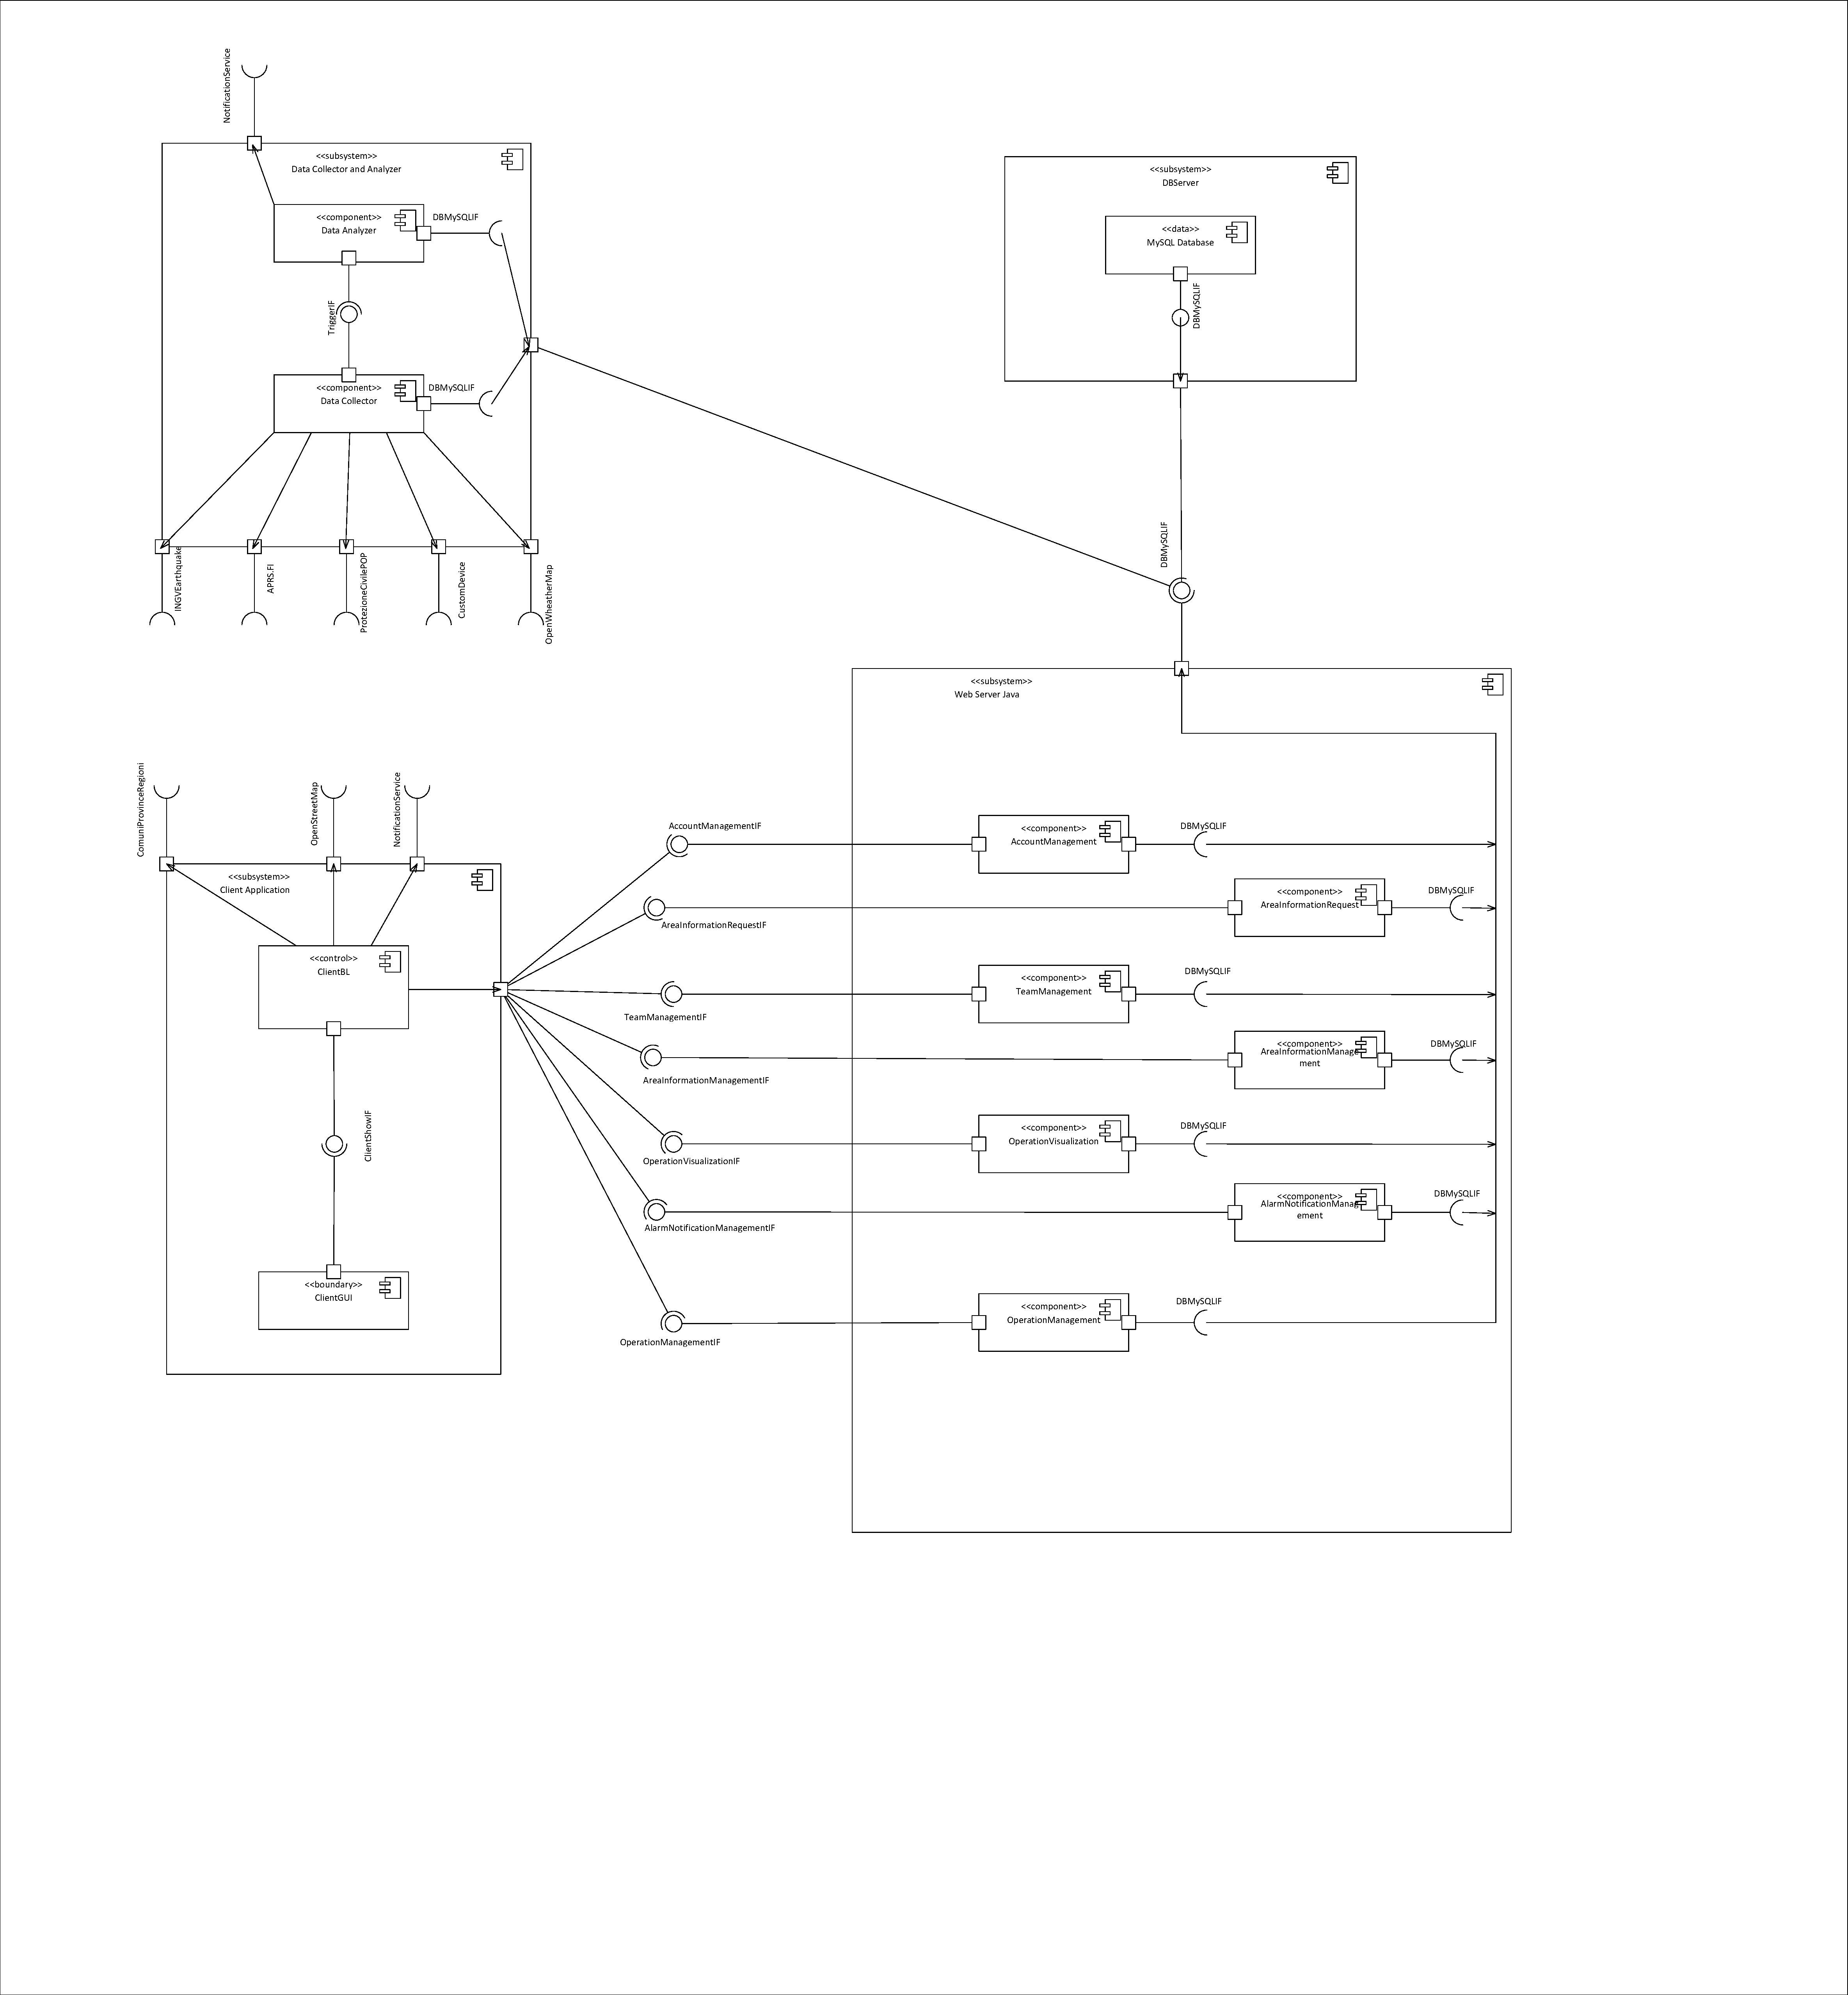
\includegraphics[width=1\linewidth]{./Iterazione 2/OtherFiles/UML - Component View}
	\caption{Component Diagram.}
	\label{fig:ComponentDiagram_iterazione2}
\end{figure}

\clearpage

\section{Class Diagram}
Di seguito sono riportate le specifiche delle strutture dati \texttt{UserDTO} e \texttt{TeamDTO} (\Fig\ref{fig:ClassDiagramDTO_iterazione2}) inserite nel server. Esse sono utilizzate per definire il formato dei dati scambiati tra l'applicazione client e applicazione server. In particolare, grazie alla direttiva \texttt{@JsonProperty(access, JsonProperty.Access.WRITE\_ONLY)} fornita da Spring, il campo \texttt{password} presente in \texttt{UserDTO} non viene mai inviato dal server al client, ma viene valorizzato dall'app client solamente durante l'inserimento di un nuovo utente.  

\begin{figure}[h!]
	\centering
	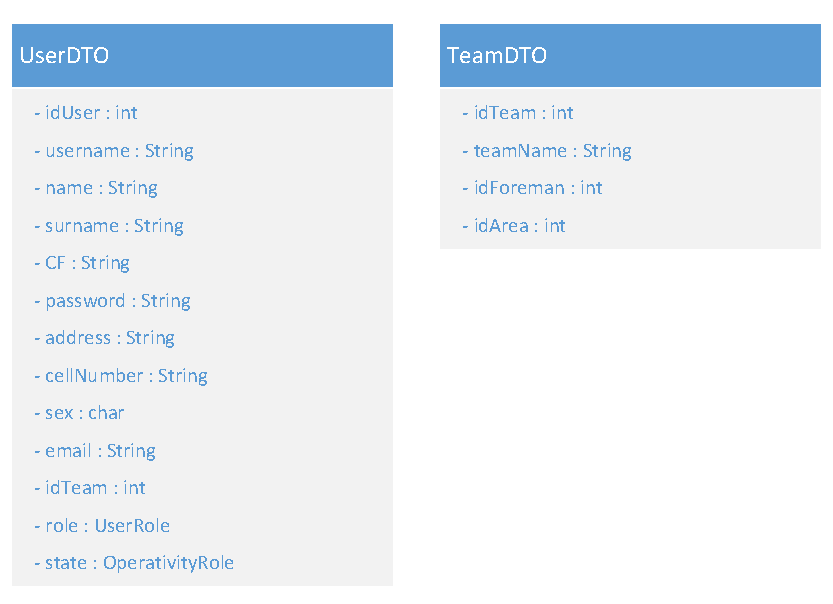
\includegraphics[width=0.8\linewidth]{./Iterazione 2/OtherFiles/DTOSpecification}
	\caption{Class Diagram \texttt{UserDTO} e \texttt{TeamDTO}}
	\label{fig:ClassDiagramDTO_iterazione2}
\end{figure}

\clearpage

\section{Interface and Package Diagram}
Nella \Fig\ref{fig:InterfaceDiagram_iterazione2} è rappresentato il diagramma delle interfacce e dei package, nel quale è stata specificata anche la firma delle interfacce introdotte nell'iterazione 2.

\begin{figure}[h]
	\centering
	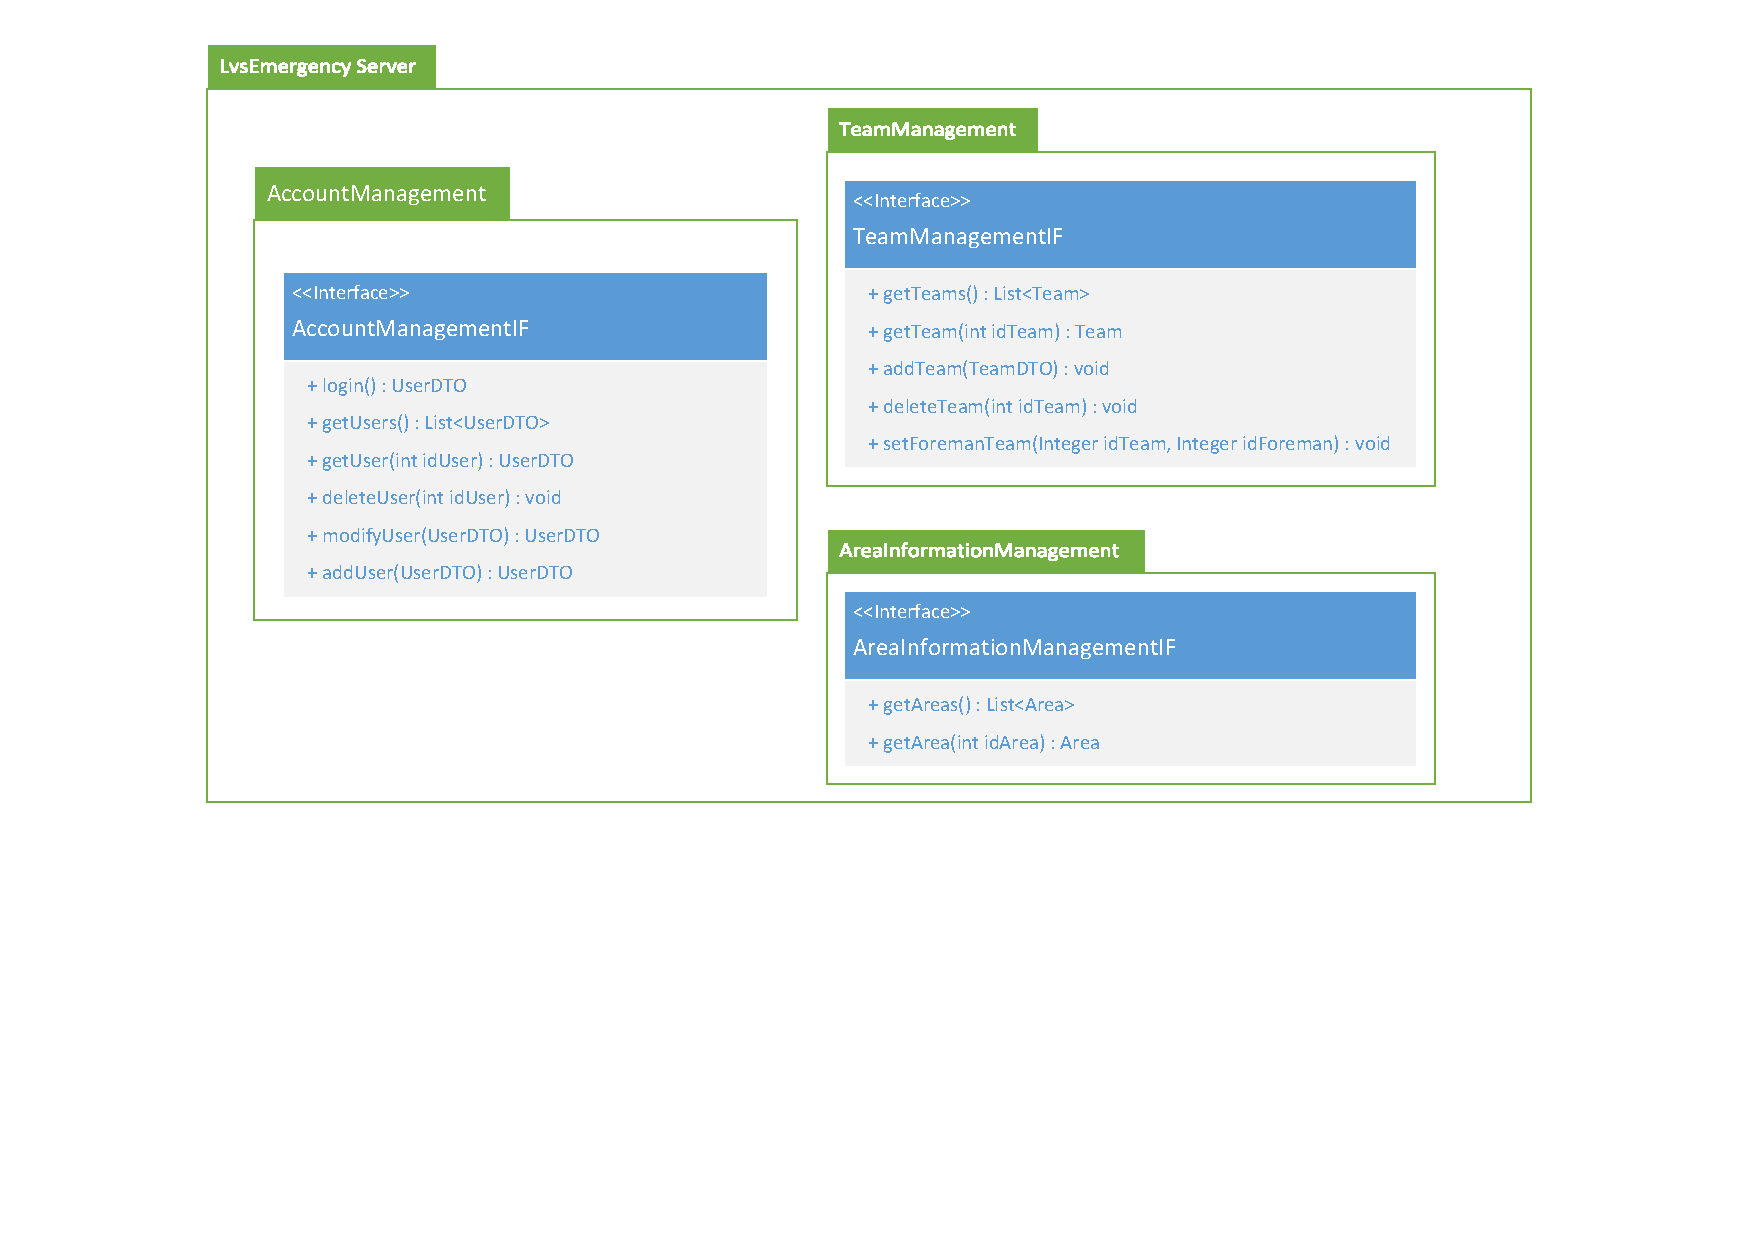
\includegraphics[width=1\linewidth]{./Iterazione 2/OtherFiles/UML - Interface Diagram}
	\caption{Interface and Package Diagram.}
	\label{fig:InterfaceDiagram_iterazione2}
\end{figure}
